\chapter{Návrh a implementace}

\section{Pravidla hry}\label{pravidla}

Fantom i detektivové mají svůj balíček žetonů, pomocí kterých můžou využívat různé dopravní
prostředky pro pohyb po mapě. Žetony jsou nepřenosné.

Pozice v mapě jsou spojené barevnými čarami, které představují trasy
jednotlivých dopravních prostředků. Černá barva představuje drožku,
zelená taxi a červená tramvaj. Tah končí přesunem pomocí dopravního
prostředku na nejbližší místo po trase. Lze pouze využívat dopravní
prostředky zvýrazněné po kliknutí na tlačítko s daným dopravním
prostředkem za předpokladu, že hráč disponuje příslušným žetonem.
Detektivové mají omezený počet žetonů. Při každém tahu odevzdává
detektiv Fantomovi žeton odpovídající zvolenému dopravnímu prostředku.
Fantom v každém svém tahu použitý žeton ukáže. Fantom se v předem daných kolech objevuje.

\subsection{Cíl hry}\label{cuxedl-hry}

Detektivové zvítězí, podaří-li se některému dorazit na místo (pozici),
kde se Fantom ukrývá. Naopak podaří-li se Fantomovi unikat až do závěru
hry, stává se vítězem.
\section{Má implementace ISMCTS}\label{sec:impl}
Má implementace umělé inteligence využívá Monte Carlo techniky v algoritmu Information Set Monte Carlo Tree Search (ISMCTS).

Celý algoritmus ISMCTS, \cref{subsub:ismcts}, je zapouzdřený v generické třídě, očekává třídu pro stav hry a třídu pro akci. Třída pro ISMCTS dále definuje dvě další třídy: vrchol a samostatný strom. 

\subsection{Vrchol}
Třída pro pomocný vrchol na budování stromu pro prohledávání si ukládá potřebné informace ohledně stavu hry, který reprezentuje, statistiky pro samostatné Monte Carlo techniky a odkaz na potomky ve stromě. Přímo si udržuje odkaz na stav hry. Informace potřebné pro fungování ISMCTS jsou počet návštěv, počet výher, který hráč hraje a jestli se jedná o informační set (jestli je počet možných historií větší než jedna) či nikoliv. Odkaz na potomky si drží pomocí slovníku, kde klíčem je vždy akce a hodnotou je vrchol představující následující stav po zahrání dané akce. Kromě toho ještě má odkaz na třídu s popisem hry - přechody mezi stavy ve hře, ohodnocení stavu, možné akce.

\subsection{Strom}
Strom udržuje v kořeni vrchol představující počáteční stav hry, se kterým byl vytvořen. Nemusí se jednat o přímo počáteční stav hry, ale pouze určité podhry. Vnitřně si udržuje generátor náhodných čísel pro simulování a explorační parametr (UCT z formule \ref{eqv:UCT}).

\subsection{Monte Carlo Tree Search}
Třídy pro vrchol a strom jsou zapouzdřené do jedné třídy, která je generická. Dostane typy pro stav hry a pro akce. Definuje také hlavní funkce pro fungování MCTS, \cref{sub:mcts}.


\subsection{Stav hry}
V každém vrcholu stromu je uložený stav hry, který vrchol reprezentuje. Stav popisuje všechny důležité informace ohledně hráčů. Mezi důležité informace spadají pozice všech hráčů. Jelikož ale Fantomova pozice nemusí být z pohledu detektivů známá, jsou-li na tahu detektivové, znají pouze množinu možných pozic Fantoma. Pozice detektivů jsou vždy známé. Důležitou součástí jsou žetony. Žetony hráčů jsou veřejné. Kromě informací o pozicích a žetonech si stav udržuje aktuální kolo a kdo je na tahu.    

\subsection{Akce}
V MCTS se buduje strom, ve kterém hrají dva hráči - Fantom a detektivové (jako celek), proto jedna akce je buď pohyb Fantoma nebo pohyb všech detektivů. Struktura představující akci pouze obsahuje seznam pohybů všech postav hráče - pro Fantoma pouze jedné, pro detektivy podle jejich počtu. Pohyb je reprezentovaný strukturou obsahující novou pozici na mapě - číslo vrcholu, a použitý dopravní prostředek. 

\subsection{Popis hry}
Poskytuje přechody mezi stavy a všechny možné akce pro daný stav, případně počet takových akcí. Pro terminální stavy vrací odměnu. Pro účely MCTS má také funkci, která z možných akcí vrací jednu náhodnou s uniformní distribucí.

\subsection{Hráči}
Pro implementaci umělé inteligence je nutné splňovat připravené rozhraní. 
Samostatní hráči si při hře pouze udržují aktuální informace o stavu hry. Ve svém tahu vytvoří novou instanci MCTS stromu s kořenem v aktuálním stavu. Pomocí třídy MCTS spustí simulaci na předem stanovený čas, případně počet iterací. Po doběhnutí algoritmu pouze vrátí správnou akci. V případě detektivů je situace lehce složitější, jelikož MCTS vrací seznam akcí všech detektivů. Detektivové si tedy zjistí všechny tahy dopředu a postupně je vrací.

\subsection{Simulátor}
Simulátor nabízí možnost simulování jednoho kola či celé hry. Hlavní úkol je rozumným způsobem reprezentovat pravidla hry - legální možnosti tahů, informování hráčů o tazích protihráče, kontrola konce hry.  

\section{Implementace hry}

\subsection{Unity}
Unity je moderní herní engine. Poskytuje možnosti vývoje 2D i 3D her. Pro vývoj her obsahuje i fyzikální engine či zvukový engine. Do scén se dají vkládat objekty, které můžou obsahovat různé komponenty. Kromě komponent na vykreslování, kolize a další, je možné k objektu přiložit i skript. Skripty se často píší v jazyce C\#. Přidávají objektu další funkcionalitu a chování. 

\subsection{Logika hry}
Je to hlavní a nejobsáhlejší třída, obstarává průběh hry. Na začátku hry načte potřebné informace z config souboru a nastaví kameru. Poté hráčům poskytne důležité informace jako počet žetonů a počet detektivů. Po vyrenderování mapy hra začne a spustí se funkce pro průběh hry (game loop). 
Game loop obsahuje nekonečný cyklus, kde jeden průběh simuluje jedno kolo hry. V každém kole se aktuálního hráče zeptá na tah, zkontroluje validitu tahu a aktualizuje stav hry. O novém stavu hry jsou oba hráči informování. Game loop je přerušen skončením hry. Hra skončí ve prospěch Fantoma, pokud trvá déle než je stanovená délka hry, pro detektivy, pokud stojí jakýkoliv detektiv na stejné pozici jako Fantom. Když hra neskončila, spustí se další iterace. 

\subsection{Pomocné skripty}
Značná část skriptů v souborech hry se stará o pomocné struktury nebo funkčnost grafického rozhraní. Vývojové prostředí Unity nabízí užitečné prvky jako např. tlačítko, textové pole, ale i složitější jako scrollovací okno. Každému takovému prvku je třeba doplnit funkčnost, například pro tlačítka při kliknutí/držení/přejetí myší. Zvolil jsem způsob pomocí připraveného skriptu se správnými objekty a funkcemi. Další z užitečných skriptů se stará o kameru, přidává možnost posouvat ji pomocí šipek a přibližovat či oddalovat pohled, jiný řeší renderování mapy a hráčů.

\subsection{Fantom}
\label{sub:fantomai}
Ve hře je také přidaná základní implementace umělé inteligence pro hráče Fantoma.
Využívá pouze heuristiky pro určení nejlepšího pohybu. Daná heuristika pro každý možný pohyb (nový vrchol) Fantoma určí hodnotu a poté vybere tah s maximálním ohodnocením. Pro ohodnocení vrcholu se z něj na mapě zavolá prohledávání do šířky (BFS) a hledá se nejkratší cesta, kterou se jakýkoliv detektiv může dostat na daný vrchol. Myšlenkou heuristiky tedy je vybrat takový vrchol, který je nejdál od nejbližšího detektiva. Nesnaží se přemýšlet a odhadovat další kola, ale pouze najít aktuální, v nějakém směru nejlepší tah. V prvním tahu, když si hráči volí pozice, nevyužívá heuristiky a pouze si vybere náhodný vrchol na mapě.

\subsection{Detektivové}
\label{sub:detectivesai}
Hra obsahuje i jednoduchou implementaci hráče za detektivy. V deskové hře za detektivy může hrát více různých hráčů. Předpokládá se určitá úroveň spolupráce mezi hráči - mají společný cíl a nezáleží na tom, který detektiv přímo dopadne Fantoma. Z hlediska umělé inteligence dává smysl reprezentovat takovou skupinu hráčů jako jednoho, který ovládá všechny figurky a snaží se s jakoukoliv dopadnout Fantoma. 
Využívá základní heuristiky. Když je detektiv na tahu, vybere si vrchol který je na nejkratší cestě k pozici, kde si myslí, že se Fantom nachází. Nejkratší cesta je hledána pomocí prohledávání do šířky a hledá pouze cesty, pro které má detektiv dostatek žetonů. Nesnaží se nijak vyvodit Fantomovu aktuální pozici z dostupných informací, ale pouze si ji vždy aktualizuje ve chvíli, kdy se Fantom ukáže. Detektivové tedy směřují na poslední Fantomovu viděnou pozici. V prvním kole se zvolí náhodná pozice pro každého detektiva, samozřejmě tak, aby nestáli na stejných pozicích.

\subsection{Interface AI}
Pro možnost rozumného rozšiřování hry o jiné implementace hráčů, Fantoma i detektivů, je připravené rozhraní pomocí interface v jazyce C\#, které musí takový hráč splňovat. Zdrojový kód s třídou splňující daný interface stačí umístit mezi soubory hry k ostatním skriptům. Hra automaticky nalezne všechny vhodné třídy a poskytne možnost vybrat si, které budou hrát za Fantoma a detektivy.

Náhled na samotný interface \ref{lst:interface}. Interface pro jazyk C\# používá následující funkce:


\begin{lstlisting}[language={[Sharp]C}, label={lst:interface}, caption={Definice rozhraní pro hráče}]
public interface IFantom : IPlayerBase { }

public interface IDetectives : IPlayerBase { }

public interface IPlayerBase : 
IPlayerBase<GameGraphScript,GameNodeScript> { }

// Base interface for all player types
public interface IPlayerBase<MapType, NodeType>
    where MapType : IMap<NodeType>
    where NodeType : INode
{
    // Called when the player's move is valid
    public void PlayIsOK(Move lastMove);

    // Synchronously gets the player's move
    public Move GetMove();
    // Asynchronously gets the player's move
    public Task<Move> GetMoveAsync();

    // Sets the available transport tokens for the player
    public void SetTransports
        (Dictionary<Transport, int> transports);
    // Sets the available transport tokens for the opponent
    public void SetOpponentTransports
        (Dictionary<Transport, int> transports);

    // Factory method to create an instance of the player
    public static IPlayerBase CreateInstance(MapType ggs)
        => throw new NotImplementedException();

    // Called when the opponent makes a move
    public void OpponentMove(Move move);
}
\end{lstlisting}


\subsubsection{Konfigurace}
Při spouštění hry se načtou základní parametry ovlivňující různé vlastnosti a chování hry. Konfigurační soubor je uložen ve formátu JSON pod názvem "config.json" v souborech hry. Samostatný soubor je rozdělený na tři části, kde každá obsahuje parametry k určité části hry.  

První část obsažená v položce "graph" udává parametry ovlivňující generování mapy. Generování ovlivňují parametry "Rows" a "Columns" udávající počet řádků a sloupců, a tři parametry obsahující pravděpodobnosti měnící generování: "probOfKeepeingNode", "probTaxi" a "probTram", jejichž použití je více přiblíženo u popisu samostatného generování.

Druhá část je pod položkou "camera". Nachází se v ní parametry, které udávají chování kamery. Mezi parametry patří "moveSpeed", "zoomSpeed", "minZoomDistance" a "maxZoomDistance", kde první parametr ovlivňuje rychlost pohybu kamery při používání šipek, druhý rychlost přibližování pomocí kolečka na myši a poslední dva pouze určují maximální a minimální přiblížení.  

Třetí část je pro průběh hry nejdůležitější. V souboru je pod názvem "game". Pod parametry spadá "fantomVisibleTurns", který obsahuje seznam kol, kdy se Fantom zjeví, "fantomTokens" a "detectiveTokens" obsahující seznam dvojic dopravní prostředek a počet žetonů pro určení počátečních žetonů všech hráčů, "numberOfTurns" nastavující délku hry, "aiDelays" pro určení minimální délky tahu hráče hraného umělou inteligencí v milisekundách a "animationSpeed", který nastavuje rychlost animace hráče při přesunu na novou pozici. 

Pokud soubor není nalezen, využije se základní, předem připravené nastavení zabudované ve hře.


\subsection{Mapa}
\subsubsection{Vrchol mapy}
Třída vrchol v sobě obsahuje důležité informace ohledně mapy. Pamatuje si dopravní prostředky, které zde mají zastávku, a vrcholy spojené trasami dopravních prostředků. Poskytuje možnost nastavit a upravit vzhled (sprite) podle zastávek dopravních prostředků a zvýrazňování (naznačení možného přesunu na daný vrchol při kole hráče). Implementuje základní funkce zlehčující práci. 

\subsubsection{Graf}
Hlavní položka je seznam (list) vrcholů. Dále obsahuje odkaz na generátor map. Při generování grafu se buď vygeneruje nová náhodná mapa nebo, pokud je vybraná, se načte uložená mapa. Při vytvoření správně nastaví vzhled (sprite) a vlastnosti každému vrcholu. Přidává další pomocné funkce, mezi které patří i jednoduchá implementace prohledávání do šířky. 


\subsubsection{Generování mapy}
Hra kromě načtení existující mapy nabízí možnost vytvoření nové náhodně vygenerované mapy. Při inicializaci generátoru mapy se načtou potřebné parametry z~config souboru. 

Mapa je generovaná jako mřížka s daným počtem řádků a sloupců - parametry "Rows" a "Columns". V mřížce každý možný vrchol s pravděpodobností danou parametrem "probOfKeepeingNode" přežije, jinak je smazaný z mřížky. Nyní má mřížka díry. Každému vrcholu se nyní přiřadí dopravní prostředky, které skrz něj budou procházet. Drožka prochází každým vrcholem a ostatní dopravní prostředky se přiřadí dle pravděpodobností z konfiguračního souboru, taxi dle "probTaxi" a tramvaj dle "probTram". Pro vytvoření hran se prochází znovu všechny vrcholy a pro každý přiřazený dopravní prostředek se pomocí prohledávání do šířky v okolí hledají jiné vrcholy obsahující tento dopravní prostředek, které se spojí hranou.

Mapu je možné nechat uložit do formátu JSON pro případné znovupoužití. Při ukládání se zapamatují důležité informace o vrcholech, podle kterých se dá mapa znovu připravit. 

\subsection{Uživatelské rozhraní}

Uživatelské rozhraní hry je připraveno s jednoduchostí v mysli. Vše je přímočaře pojmenované. 

\subsubsection{Hlavní menu}

Hlavní menu na Obrázku~\ref{fig:main_menu} obsahuje několik důležitých prvků. 

Na levé straně obrazovky jsou možnosti výběru hráčů za Fantoma a detektivy. Ve hře jsou připravené tři různé možnosti hráče za Fantoma i detektivy, viz Obrázek~\ref{fig:player_selector}, ale hra podporuje možnost přidání hráčem vytvořené umělé inteligence splňující správné rozhraní. Mezi připravené možnosti u detektivů spadá "DetectiveReal", který umožňuje detektivy ovládat ručně při hře, "DetectiveAI" je umělá inteligence využívající heuristiky pro rozhodování a "DetectivesAIMCTS" implementující ISMCTS pro rozhodování. Pro Fantoma jsou obdobné. 

Na pravé straně se nachází tři tlačítka. Tlačítko "UKONČIT" pouze vypne spuštěnou hru. Při kliknutí na tlačítko "MAPY" se zobrazí možnost výběru uložených map ve formátu JSON v souborech hry. Po vybrání mapy se v následující hře použije. Pokud žádná mapa není zvolená, vygeneruje se náhodná. Poslední tlačítko "HRÁT" spustí hru se zvoleným nastavením hráčů a mapy.

\begin{figure}[h] % 'h' stands for 'here'. You can use other options like 't' for top, 'b' for bottom, etc.
  \centering
  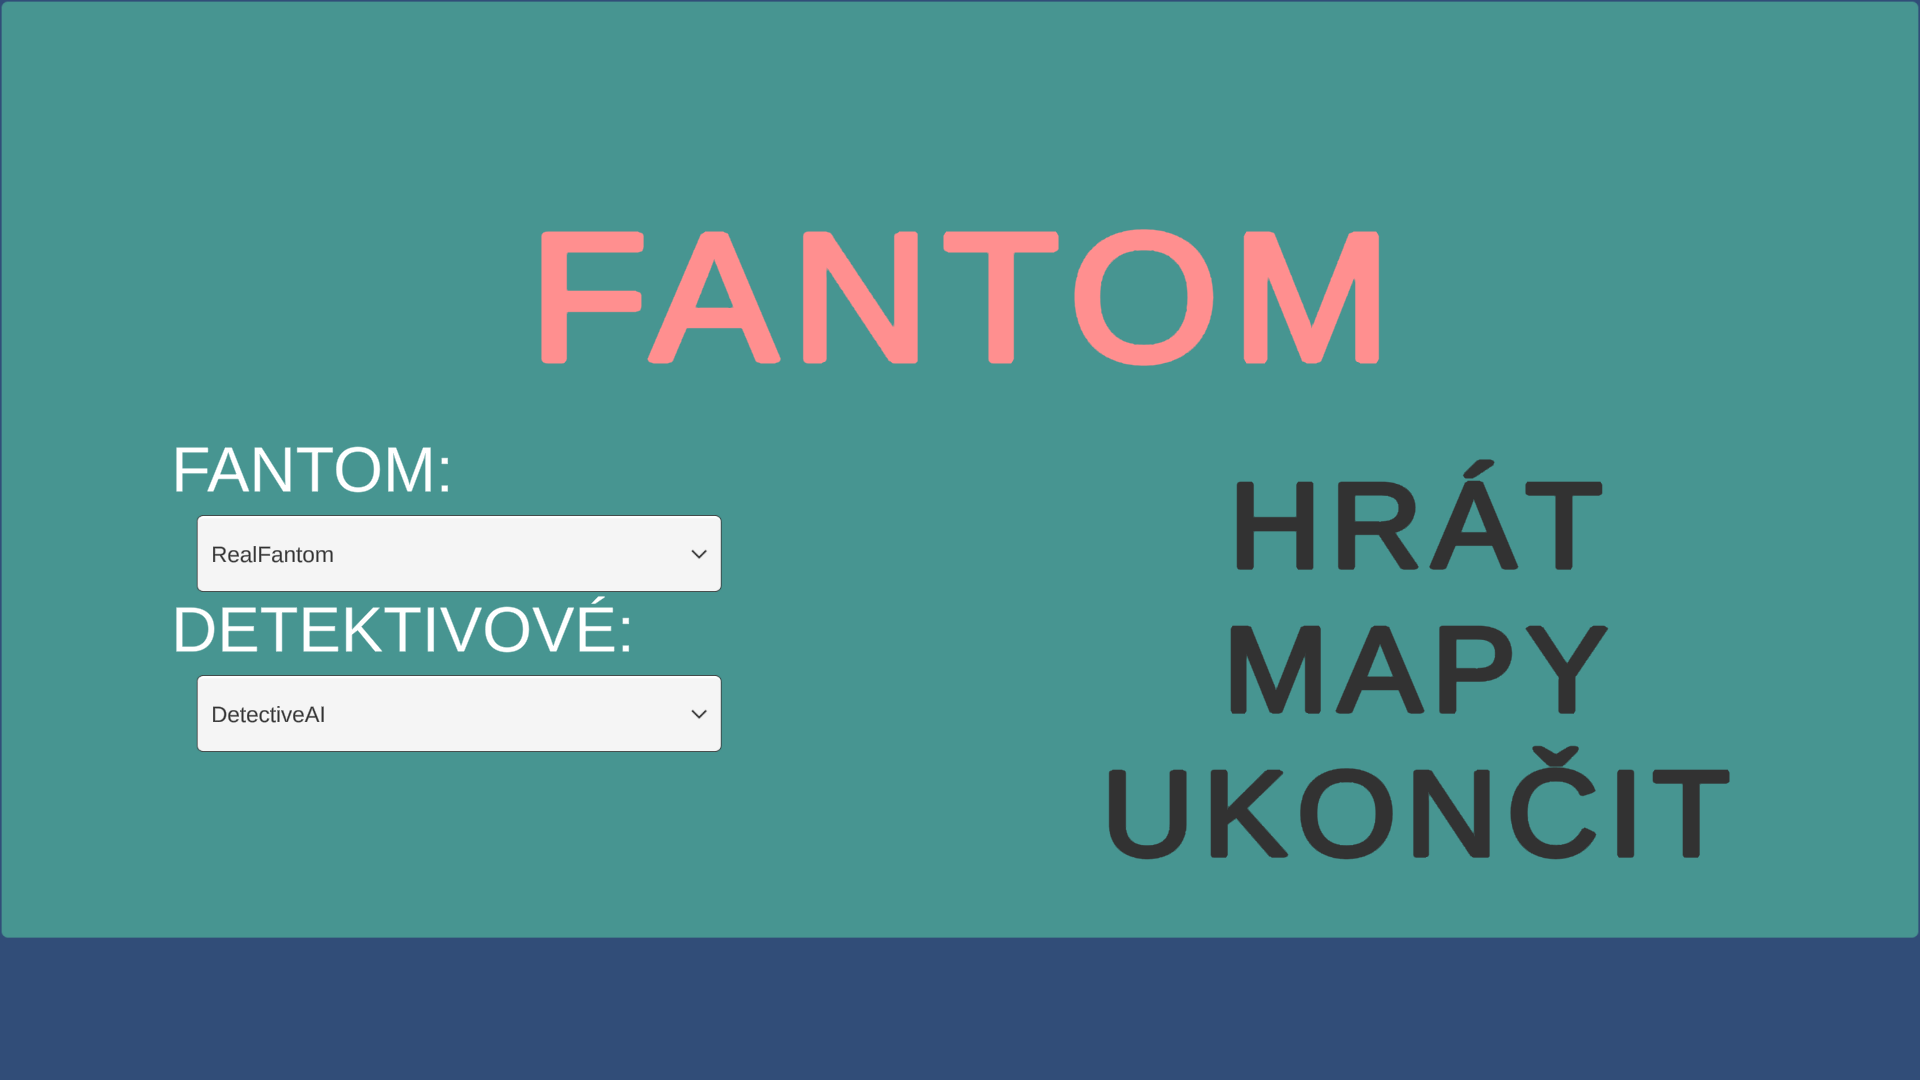
\includegraphics[width=1\textwidth]{main_menu.png}
  \caption{Hlavní menu}
  \label{fig:main_menu}
\end{figure}

\begin{figure}[h]
  \centering
  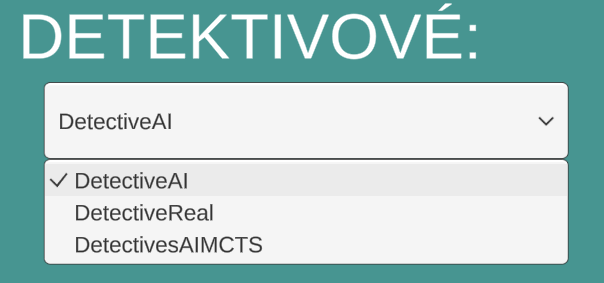
\includegraphics[width=1\textwidth]{player_selector.png}
  \caption{Výběr hráče}
  \label{fig:player_selector}
\end{figure}
\clearpage
\subsubsection{Herní obrazovka}

Při hře vidí hráč mapu hry a důležité informace o hře viz Obrázek~ \ref{fig:ingame_view}. Vlevo nahoře se nachází aktuální kolo, kdo je na tahu (Fantom či detektiv) a tlačítko "Schovat Fantoma", které pouze zneviditelní či naopak ukáže Fantoma, je určeno pro hraní dvou lidí proti sobě, pro hraní s umělou inteligencí se nedoporučuje využívat. Vlevo dole jsou dvě tlačítka, "Všechny žetony", které zobrazí tabulku s počtem aktuálních žetonů dopravních prostředků pro každého hráče, a "Fantom tahy" zobrazující historii Fantomových tahů, která se objeví vpravo, aktuálně je zobrazená. Vpravo dole jsou tři tlačítka pro dopravní prostředky, pomocí kterých se hráč, zvolil-li si ovládání Fantoma či detektivů a je právě na tahu, vybírá dopravní prostředek na cestování. Po zvolení dopravního prostředku se zvýrazní možné tahy žlutým kruhem (ukázka po zvolení Tramvaje na Obrázku~\ref{fig:ingame_view})

\begin{figure}[h]
  \centering
  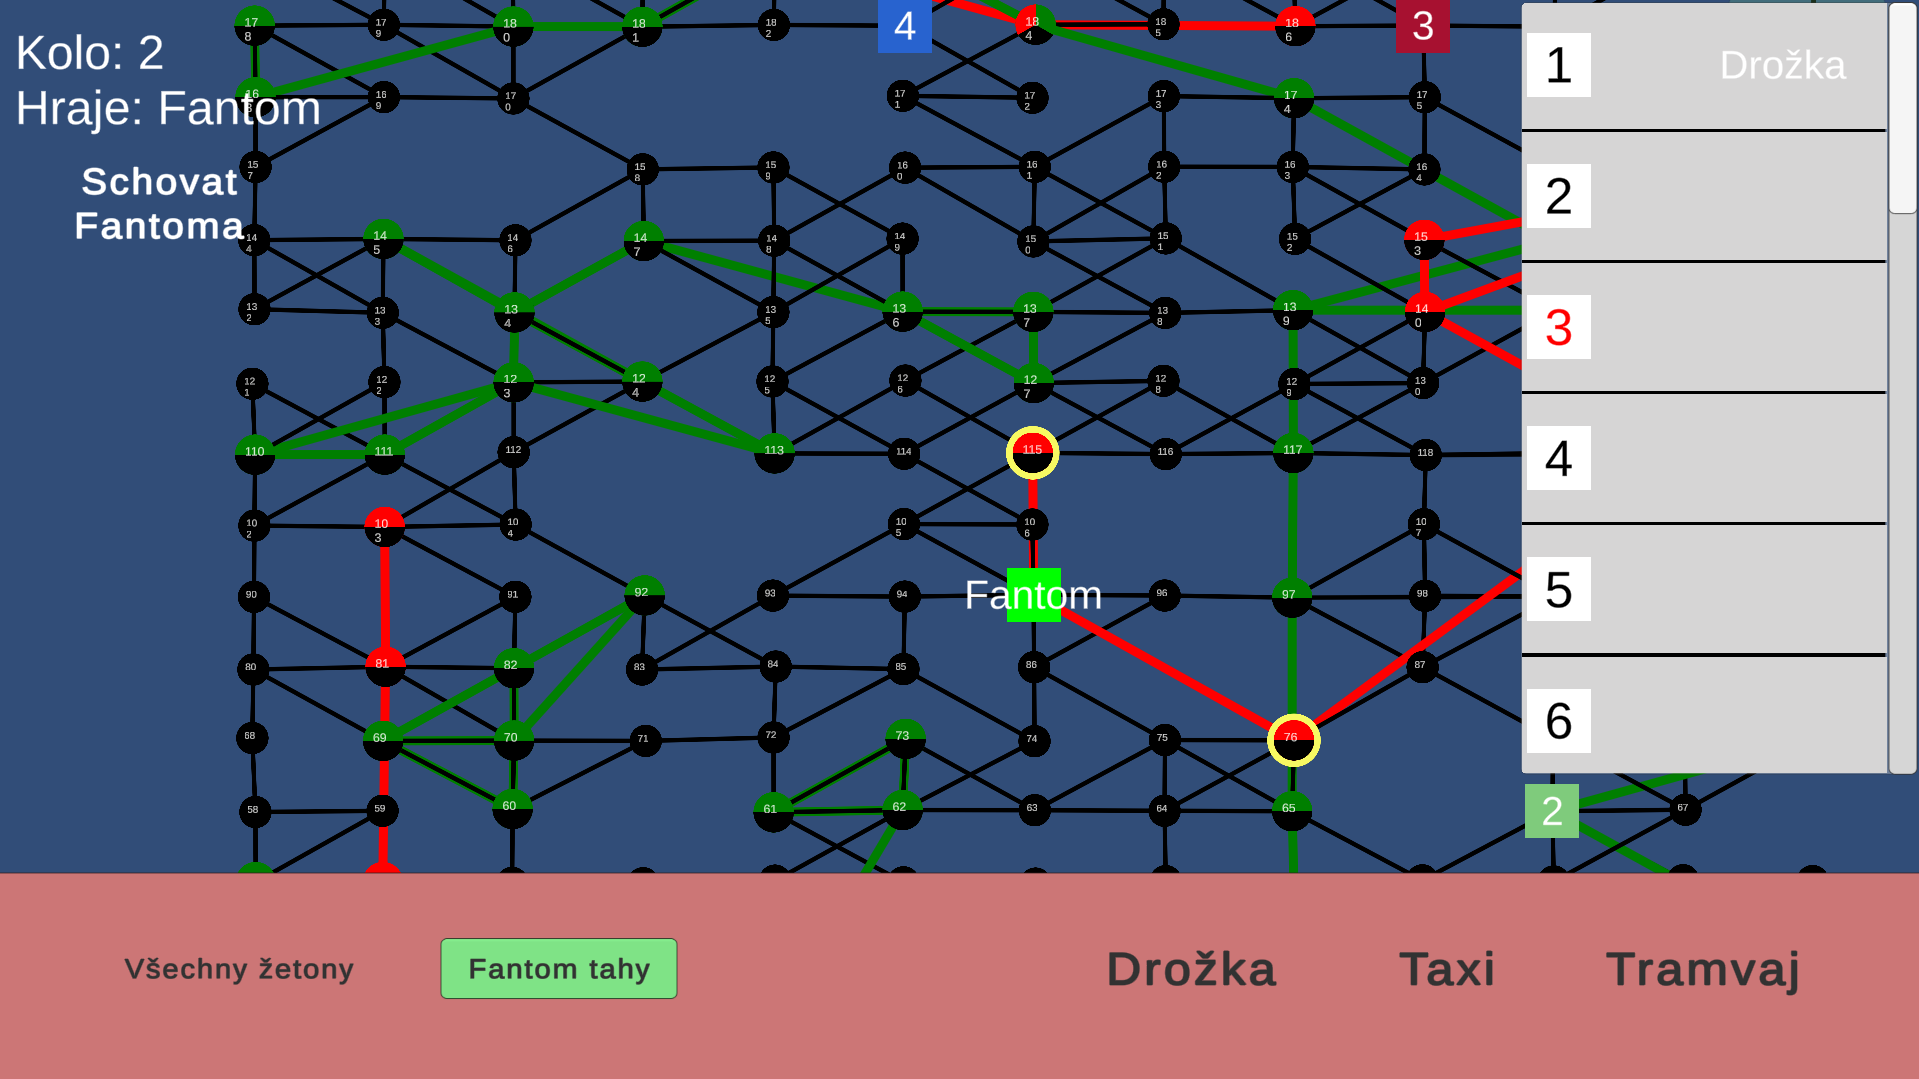
\includegraphics[width=1\textwidth]{ingame_view.png}
  \caption{Pohled při hře, vpravo historie tahů Fantoma}
  \label{fig:ingame_view}
\end{figure}
\clearpage
\subsubsection{Konec hry}

Po dohrání hry se objeví menu nabízející ukončení hry pomocí "UKONČIT", hrát znovu pomocí "HRÁT ZNOVU" a uložení mapy do správného JSON formátu mezi soubory hry pomocí "ULOŽIT MAPU" (Obrázek~\ref{fig:end_menu}).

\begin{figure}[h]
  \centering
  
\includegraphics[width=0.8\textwidth]{end_menu.png}
  \caption{Menu po dohrání hry}
  \label{fig:end_menu}
\end{figure}

\section{Instalace hry}

Vše potřebné zajistí k práci přiložený FantomInstaller.exe. Vytvoří novou složku s hrou ve stejné složce, ve které se nachází. Hra je spustitelná pomocí souboru ``Fantom.exe''.
